\section{The Iteration Keyword}
\label{sec:iteration}

Our approach to removing induction variable state is to introduce a
new language construct that directly represents the basis of induction
variable state. The construct maintains a value indicating how often
the corresponding filter has been invoked. 

This approach was chosen over implementing a system to automatically
recognize induction variable usage in filter construction. The
approach of automatic analysis would require detecting induction
variables defined in the filter. The simplest form of this analysis
would idiomatically detect a variable modified by a statement similar
to \texttt{var=var+1}. Very few iteration filters (outside of source
filters) use induction state in this limited capacity. Consider
Figure~\ref{fig:wc-example}(a), where the induction variable is
incremented at each iteration step, until a certain threshold value at
which it will reset. This pattern is very common in programs that use
induction filters. MPD and FIRBank use this technique to iterate
across a provided array one element per iteration step. To ensure
consistency between iteration steps, the automatic analysis is
required to detect these types of updates as well.

% \begin{figure}[t]
% {\eightpoint
% \begin{verbatim}
% float->float filter WeightCalc(int n)
% {
%   float[n] window;
%   int windowPos;

%   ...

%   // the input stream is multiplied with the weights
%   work push 2 pop 2
%   {

%     push(pop() * window[windowPos]);
%     push(pop() * window[windowPos]);

%     windowPos++;
%     if(windowPos >= n)
%     {
%       windowPos = 0;
%     }
%   }
% }
% \end{verbatim}
% \caption{MPD filter that multiplies stream values with weights.\protect\label{fig:weight-calc}}}
% \end{figure}


\begin{figure*}[t!]
\centering
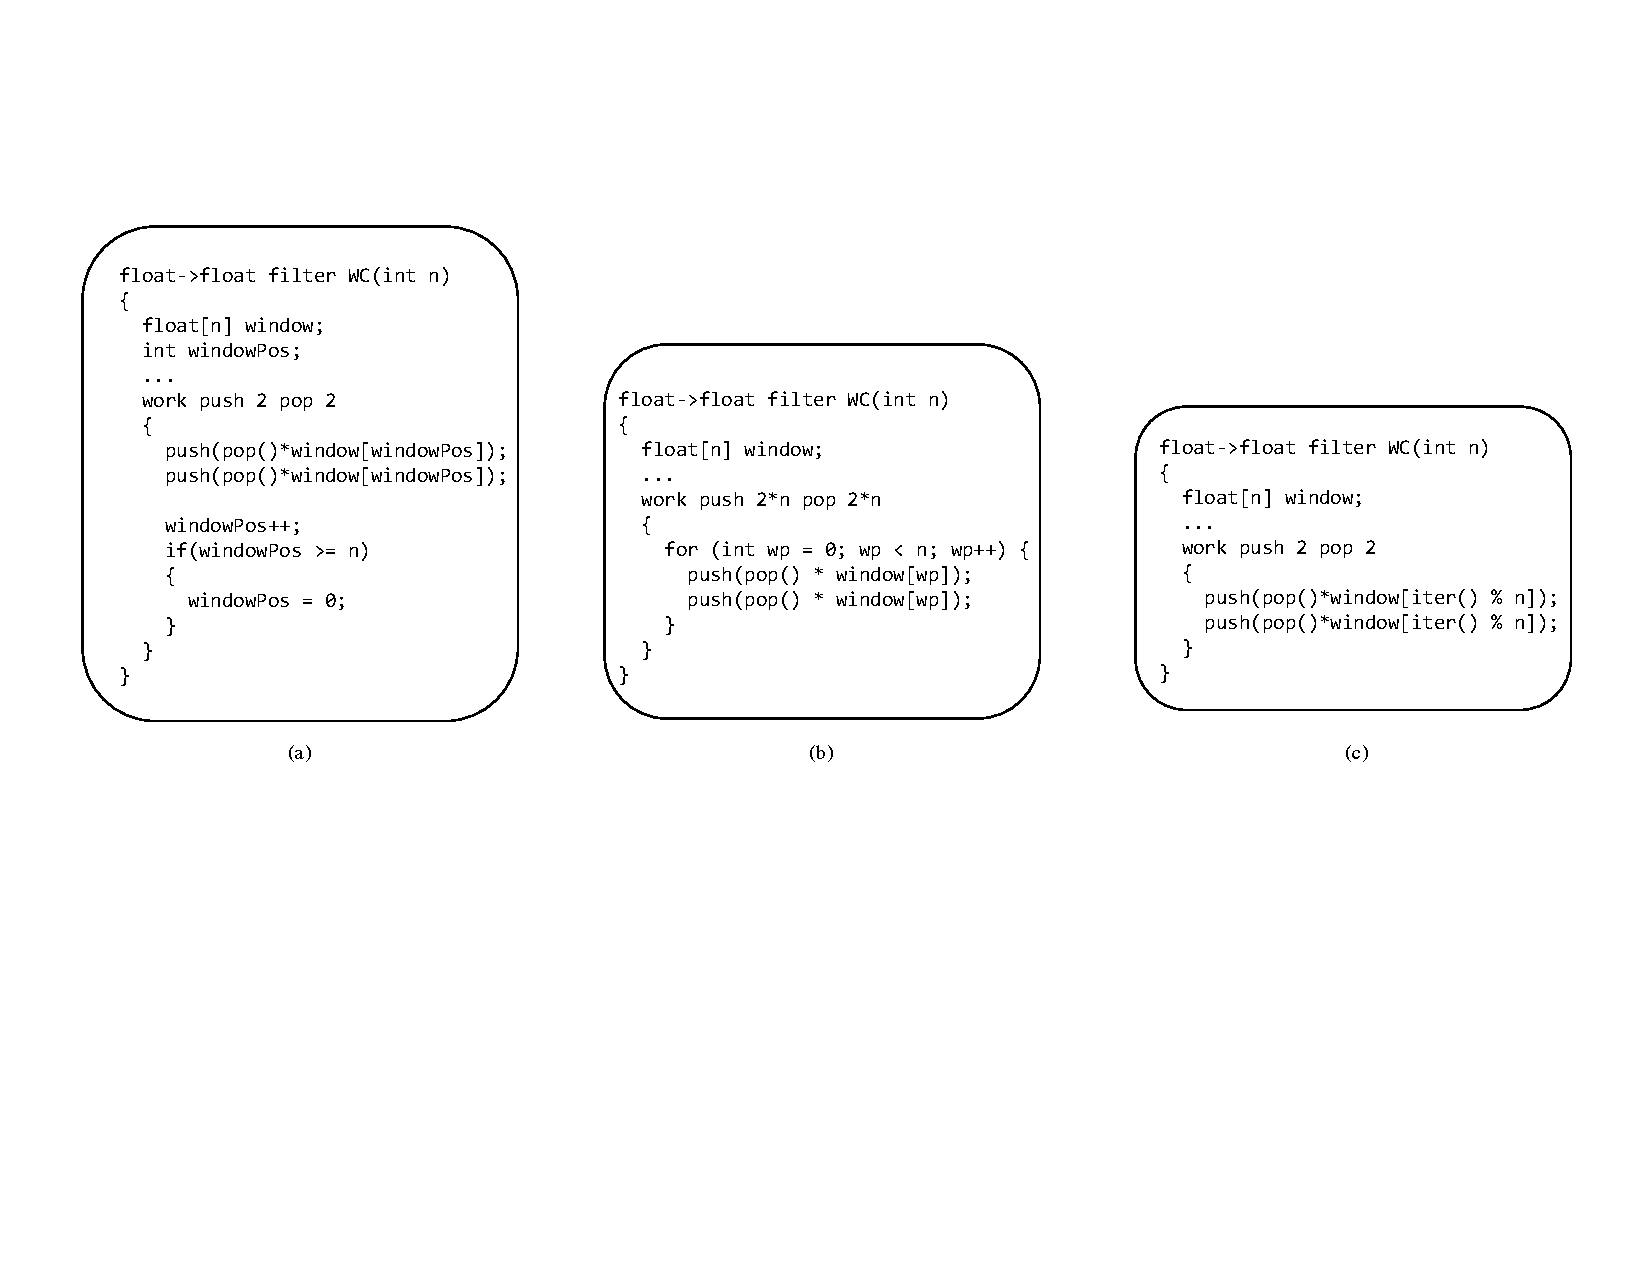
\includegraphics[width=6.5in]{figures/weights-calc-example.pdf}
\caption{Three versions of the weights calculation filter from Medium Pulse Dopler (MPD) (a) is the original filter with explicit induction variable state.  (b) is a coarsened version without state. (c) is a version that utilizes the {\tt iter()} keyword to avoid state.\protect\label{fig:wc-example}}
\end{figure*}


A filter may have multiple induction variables that are dependent on
one another in defining their values, as in the stateful filter in
Figure~\ref{fig:transform-after-twonested}. The automatic analysis
must also be able to detect incrementing statements that may not
necessarily be updated on every work call. The process of simply
detecting and identifying induction variables can potentially branch
into many cases that need to be specially implemented.

There may potentially be other special cases that must be defined into the automatic analysis.  Filters may define induction variables that start with and reset to a particular value.  Induction variables may increment by a different value other than one at each execution step.  Co-induction variables may be constructed to reset the value of other induction variables after reaching a certain value.  The different uses of induction variables may be difficult to assess.  Though the methods of using induction variables as illustrated in Figures~\ref{fig:wc-example} and~\ref{fig:transform-after-twonested} encompass many of the common use cases in the benchmark suite, slight variations in the implementation to the pattern may prevent the induction variable from being detected.

% Automatic recognition is fairly inflexible in detecting induction variable state.  The process would restrict data parallelism opportunities to only the filters that fit the implemented templates.  We instead elect to provide the user with the flexibility of defining their own derived induction values.  

It may also be difficult to detect how the induction value will be
updated, as some of the use cases described above may demonstrate. The
keyword solution has the added benefit of maintaining a value that is
predictable in its updates. The value that the keyword returns is
simply the number of times the filter has been invoked. This value is
always incremented by one at the end of every work call.

Furthermore, the approach of automatic analysis does little to
encourage programming with parallelism in mind. On inspection, user
written code will still maintain state, which actively inhibits data
parallelism opportunities. In introducing a language construct, user
written code eliminates explicitly kept state. This approach
encourages users to write code with the intention of exploiting
parallelism.


